\subsection{Architettura dei simulatori} \label{sec:architettura_simulatori}
Nonostante i simulatori non siano ufficialmente considerati parte integrante del prodotto dalla proponente, il nostro team ha scelto di dedicare alcune risorse alla progettazione di questa componente nell'ambito del progetto didattico. Inoltre, abbiamo deciso di implementare e tenere conto delle possibili logiche dei microcontrollori associati ai sensori IoT, che possono effettuare operazioni per rendere più efficiente l'intero sistema.

Nei paragrafi successivi, verrà presentata l'architettura individuata mediante l'utilizzo di diagrammi delle classi e relative descrizioni rapide. Inoltre, saranno motivate le scelte dei design pattern individuati e le decisioni progettuali rilevanti. Successivamente, per ogni classe, saranno illustrati metodi e attributi.
\subsubsection{Modulo simulatori sensori}
\begin{figure}[H]
    \centering
    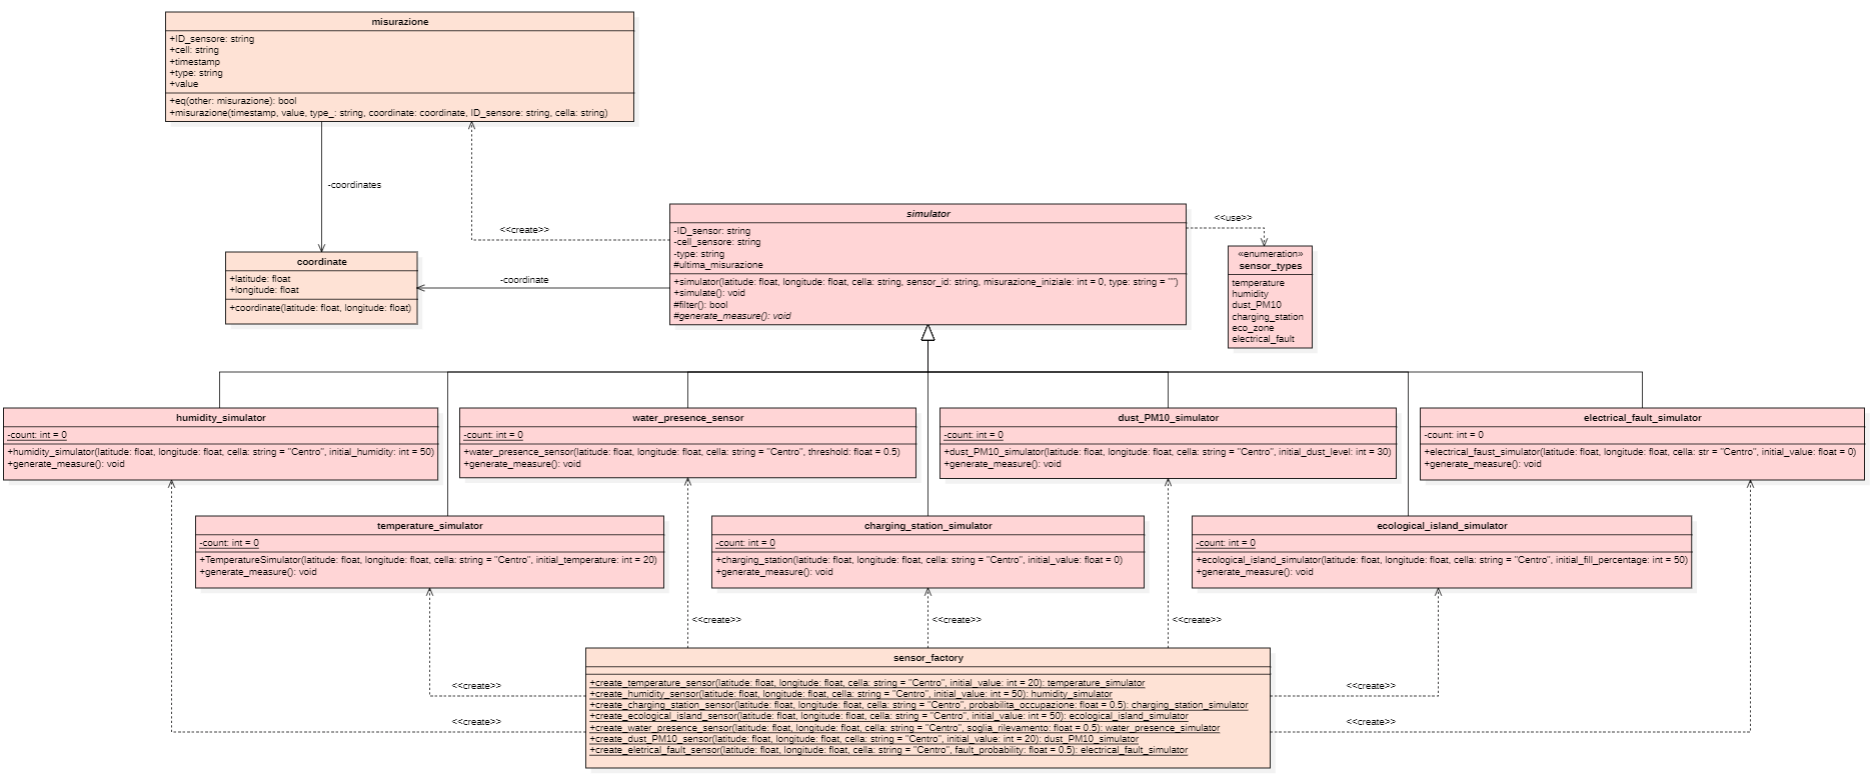
\includegraphics[width=1\textwidth]{../Images/SpecificaTecnica/simulatoriSensori.PNG}
    \caption{Modulo simulatori sensori - innovacity}
    \label{fig: fddf}
\end{figure}
Questo modulo si occupa della generazione di dati di misurazione per diverse tipologie di sensori.
In particolare sono stati implementati simulatori per i seguenti tipi di sensori:
\begin{itemize}
    \item Sensori di temperatura;
    \item Sensori di umidità;
    \item Sensori di polveri sottili PM10;
    \item Sensori di stato occupazione colonnine di ricarica;
    \item Sensori di stato riempimento isole ecologica;
    \item Sensori di presenza d'acqua;
    \item Sensori di guasto elettrico.
\end{itemize}
\paragraph{Design pattern Template Method:}

La classe astratta \textit{Simulator} implementa il design pattern \textit{Template Method}. Il metodo \textit{simulate()} fornisce lo scheletro dell'algoritmo per la generazione e la gestione delle misurazioni. Le classi concrete che estendono \textit{Simulator} implementano:
\begin{itemize}
    \item \textbf{Metodo \textit{generate\_measure()}}: per la generazione semi randomica della misurazione associata al tipo di sensore;
    \item \textbf{Metodo \textit{filter()}}: per la logica di filtrazione di misurazioni errate o non attendibili (ad esempio, negative, fuori range o consecutive troppo distanti). Il metodo \textit{filter()} offre un'implementazione di default che lascia passare ogni misurazione senza modifiche.
\end{itemize}

Il design pattern \textit{Template Method} è stato scelto per:
\begin{itemize}
    \item Permettere una facile estensione del sistema con nuovi tipi di sensori che dovranno unicamente implementare la loro logica di generazione delle misurazioni e di filtering se necessario;
    \item Standardizzare i passi per la generazione delle misurazioni, garantendo coerenza e manutenibilità del codice;
    \item Ridurre la duplicazione del codice.
\end{itemize}

Una volta ottenuto lo stato del sensore, esso viene inserito in un oggetto di tipo \textit{Misurazione}. Questo oggetto contiene informazioni di contesto come:
\begin{itemize}
    \item Identificativo del sensore;
    \item Cella della città in cui è presente;
    \item Timestamp della misurazione;
    \item Valore della misurazione;
    \item Coordinate;
    \item Tipologia di misurazione.
\end{itemize}
L'oggetto \textit{Misurazione} viene poi ritornato al chiamante che si occuperà di inviarlo al server \textit{Kafka}.
Un oggetto di tipo \textit{Simulator} verrà assegnato ad ogni \textit{SimulatorThread} che chiamerà ad intervalli regolari il metodo \textit{simulate()} ottenendo appunto la misurazione che invierà al server \textit{Kafka} tramite un modulo apposito e indipendendente.

\paragraph{Design pattern Factory:}
SensorFactory implementa il design pattern \textit{Factory} per la creazione di simulatori dei sensori.
Il pattern FACTORY è un pattern di tipo “Creazionale” secondo la classificazione della GoF.
I pattern di tipo creazionali si occupano della costruzione delle simulazioni dei sensori e delle problematiche che si possono originare, astraggono il processo di creazione degli oggetti, nascondono i dettagli della creazione e rendono i sistemi indipendenti da come gli oggetti sono creati e composti.
Il pattern Factory incapsula la creazione concreta dei sensori, consentendo al client
(l’utilizzatore) di non conoscere i dettagli.


\paragraph{Classi: metodi e attributi}
\begin{itemize}
    \item {\textbf{Classe astratta: \textit{Simulator}}}
        \begin{itemize}
            \item \textbf{Attributi}: 
            \begin{itemize}
                \item \textbf{ID\_sensor:str [private]} - Identificatore univoco del sensore.
                \item \textbf{cella\_sensore:str [private]} - Identificatore della cella del sensore.
                \item \textbf{coordinate:Coordinate [private]} - Coordinate geografiche del sensore.
                \item \textbf{misurazione: T [protected]} - Misurazione corrente del sensore.
                \item \textbf{type:str [private]} - Tipo di sensore.
            \end{itemize}
            \item \textbf{Metodi}:
            \begin{itemize}
                \item \textbf{simulate():Misurazione [public]} - Metodo principale per simulare la generazione di una misurazione.
                Si basa sul design pattern Template Method:
                \begin{enumerate}
                    \item     Chiama generate\_measure() per generare un valore di misurazione.
                    \item     Verifica con filter() se la misurazione è valida (ripete la generazione finché non lo è).
                    \item     Restituisce un oggetto Misurazione con data e ora corrente, valore misurato, tipo di sensore, coordinate e identificativo del sensore.
                \end{enumerate}
                \item \textbf{generate\_measure():None [protected]} - Metodo astratto da implementare nelle classi concrete per generare un valore di misurazione semi-casuale coerente con la tipolgia di sensore da salvare nell'attributo \textit{misurazione}.
                \item \textbf{filter():bool [protected]} - Metodo di filtro per la validazione della misurazione (implementazione di default che accetta sempre la misurazione). Può essere ridefinito nelle classi concrete per implementare la logica di filtraggio.
            \end{itemize}
            \item \textbf{Note}:
            \begin{itemize}
                \item La classe Simulator è astratta e definisce il comportamento generale della simulazione della misurazione.
                \item Le classi concrete che ereditano da Simulator devono implementare il metodo astratto generate\_measure().
                \item Il metodo filter() può essere ridefinito nelle classi concrete per implementare la logica di validazione specifica del sensore.
            \end{itemize}
        \end{itemize}
        
        
        
        
        \item{\textbf{Enumerazione: \textit{SensorTypes}}}
        \begin{itemize}
            \item \textbf{Costanti}: 
            \begin{itemize}
                \item \textbf{TEMPERATURE:str [public]} - Rappresenta la nomenclatura dei sensore di temperatura.
                \item \textbf{HUMIDITY:str [public]} - Rappresenta la nomenclatura dei sensore di umidità.
                \item \textbf{DUST\_PM10:str [public]} - Rappresenta la nomenclatura dei sensore di "polvere PM10".
                \item \textbf{CHARGING\_STATION:str [public]} - Rappresenta la nomenclatura dei sensore di stato delle colonnine di ricarica.
                \item \textbf{ECOLOGICAL\_ISLAND:str [public]} - Rappresenta la nomenclatura dei sensore di stato riempimento isole ecologica.
                \item \textbf{WATER\_PRESENCE:str [public]} - Rappresenta la nomenclatura dei sensore di presenza d'acqua.
                \item \textbf{ELECTRICAL\_FAULT:str [public]} - Rappresenta la nomenclatura dei sensore di guasti elettrici.
            \end{itemize}

            \item \textbf{Note}:
            \begin{itemize}
                \item L'enumerazione viene utilizzata per centralizzare la gestione della nomenclatura dei tipi di sensori che verrà salvata nelle misurazioni.
            \end{itemize}
        \end{itemize}
        
        
    \item{\textbf{Classe: \textit{TemperatureSimulator}}}
    \begin{itemize}
        \item \textbf{Attributi:}
    \begin{itemize}
        \item \textbf{count:int [private, static]} - Contatore statico per generare un ID univoco per ogni istanza.
    \end{itemize}
    \item\textbf{Metodi}: 
    \begin{itemize}
        \item \textbf{generate\_measure():None [protected]} - Genera una misurazione di temperatura semi-casuale e aggiorna la misurazione corrente.
    \end{itemize}
    \item\textbf{Note}:
    \begin{itemize}
        \item La classe TemperatureSimulator è una classe concreta che eredita dalla classe astratta Simulator.
        \item Il costruttore genera automaticamente un ID sensore univoco per ogni istanza.
    \end{itemize}
\end{itemize}
    \item{\textbf{Classe: \textit{HumiditySimulator}}}
    \begin{itemize}
        \item\textbf{Attributi:}
    \begin{itemize}
        \item \textbf{count:int [private, static]} - Contatore statico per generare un ID univoco per ogni istanza.
    \end{itemize}
    \item \textbf{Metodi}: 
    \begin{itemize}
        \item \textbf{generate\_measure():None [protected]} - Genera una misurazione di umidità semi-casuale e aggiorna la misurazione corrente.
    \end{itemize}
    \item \textbf{Note}:
    \begin{itemize}
        \item La classe HumiditySimulator è una classe concreta che eredita dalla classe astratta Simulator.
        \item Il costruttore genera automaticamente un ID sensore univoco per ogni istanza.
    \end{itemize}
\end{itemize}
    \item{\textbf{Classe: \textit{ChargingStationSimulator}}}
    \begin{itemize}
        \item  \textbf{Attributi}: 
    \begin{itemize}
        \item \textbf{count:int [private, static]} - Contatore statico per generare un ID univoco per ogni istanza.
    \end{itemize}
    \item  \textbf{Metodi}:
    \begin{itemize}
        \item \textbf{generate\_measure():None [protected]} - Genera lo stato della colonnina di ricarica (Occupato: True, Libero: False) basata su una probabilità di transizione.
    \end{itemize}
    \item   \textbf{Note}:
    \begin{itemize}
        \item La classe ChargingStationSimulator è una classe concreta che eredita dalla classe astratta Simulator.
        \item Implementa il metodo astratto generate\_measure() per generare una misurazione basata sulla probabilità di transizione.
        \item Il costruttore genera automaticamente un ID sensore univoco per ogni istanza.
    \end{itemize}
\end{itemize}
    \item{\textbf{Classe: \textit{DustPM10Simulator}}}
    \begin{itemize}
        \item   \textbf{Attributi}: 
    \begin{itemize}
        \item \textbf{count:int [private, static]} - Contatore statico per generare un ID univoco per ogni istanza.
    \end{itemize}
    \item    \textbf{Metodi}: 
    \begin{itemize}
        \item \textbf{generate\_measure():None [protected]} - Genera una variazione di polvere PM10 semi-casuale e aggiorna la misurazione corrente.
    \end{itemize}
    \item    \textbf{Note}:
    \begin{itemize}
        \item La classe DustPM10Simulator è una classe concreta che eredita dalla classe astratta Simulator.
        \item Il costruttore genera automaticamente un ID sensore univoco per ogni istanza.
    \end{itemize}
\end{itemize}
    \item{\textbf{Classe: \textit{ElectricalFaultSimulator}}}
    \begin{itemize}
        \item   \textbf{Attributi}: 
    \begin{itemize}
        \item \textbf{count:int [private, static]} - Contatore statico per generare un ID univoco per ogni istanza.
    \end{itemize}
    \item   \textbf{Metodi}: 
    \begin{itemize}
        \item \textbf{generate\_measure():None [protected]} - Genera lo stato di una centralina elettrica (Guasto verificato: True, Operativa: False) basata sulla probabilità di guasto.
    \end{itemize}
    \item   \textbf{Note}:
    \begin{itemize}
        \item La classe ElectricalFaultSimulator è una classe concreta che eredita dalla classe astratta Simulator.
        \item Il costruttore genera automaticamente un ID sensore univoco per ogni istanza.
    \end{itemize}
\end{itemize}
    \item{\textbf{Classe: \textit{EcologicalIslandSimulator}}}
    \begin{itemize}
        \item    \textbf{Attributi}: 
    \begin{itemize}
        \item \textbf{count:int [private, static]} - Contatore statico per generare un ID univoco per ogni istanza.
    \end{itemize}
    \item    \textbf{Metodi}: 
    \begin{itemize}
        \item \textbf{generate\_measure():None [protected]} - Genera una misurazione della percentuale di riempimento di un isola ecologica.
    \end{itemize}
    \item    \textbf{Note}:
    \begin{itemize}
        \item La classe EcologicalIslandSimulator è una classe concreta che eredita dalla classe astratta Simulator.
        \item Il costruttore genera automaticamente un ID sensore univoco per ogni istanza.
    \end{itemize}
\end{itemize}
    \item{\textbf{Classe: \textit{WaterPresenceSensor}}}
    \begin{itemize}
        \item    \textbf{Attributi}: 
    \begin{itemize}
        \item \textbf{count:int [private, static]} - Contatore statico per generare un ID univoco per ogni istanza.
    \end{itemize}
    \item    \textbf{Metodi}: 
    \begin{itemize}
        \item \textbf{generate\_measure():None [protected]} - Genera una misurazione basata sulla soglia di presenza dell'acqua (Acqua rilevata: True, Acqua non rilevata:False).
    \end{itemize}
    \item    \textbf{Note}:
    \begin{itemize}
        \item La classe EcologicalIslandSimulator è una classe concreta che eredita dalla classe astratta Simulator.
        \item Il costruttore genera automaticamente un ID sensore univoco per ogni istanza.
    \end{itemize}
\end{itemize}
    \item{\textbf{Classe: \textit{Misurazione}}}
    \begin{itemize}
        \item   \textbf{Attributi}: 
    \begin{itemize}
        \item \textbf{timestamp:datetime [private]} - Timestamp della misurazione.
        \item \textbf{value:T [private]} - Valore della misurazione.
        \item \textbf{type:str [private]} - Tipo della misurazione.
        \item \textbf{coordinates:Coordinate [private]} - Coordinate della misurazione.
        \item \textbf{ID\_sensore:str [private]} - ID del sensore che ha effettuato la misurazione.
        \item \textbf{cella:str [private]} - Cella in cui è stata effettuata la misurazione.
    \end{itemize}
    \item   \textbf{Metodi}: 
    \begin{itemize}
        \item \textbf{\_\_eq\_\_(other:Misurazione):bool [public]} - Ridefinizione dell'operatore di uguaglianza per confrontare due oggetti Misurazione.
    \end{itemize}
\end{itemize}
    \item{\textbf{Classe: \textit{Coordinate}}}
    \begin{itemize}
        \item    \textbf{Attributi}: 
    \begin{itemize}
        \item \textbf{latitude:float [private]} - Latitudine della coordinata.
        \item \textbf{longitude:float [private]} - Longitudine della coordinata.
    \end{itemize}
    \item     \textbf{Metodi}: 
    \begin{itemize}
        \item \textbf{\_\_eq\_\_(other:Coordinate):bool [public]} - Ridefinizione dell'operatore di uguaglianza per confrontare due oggetti Coordinate.
    \end{itemize}
\end{itemize}
    \item{\textbf{Classe: \textit{SensorFactory}}}
    \begin{itemize}
        \item    \textbf{Metodi}: 
\begin{itemize}
    \item \textbf{create\_temperature\_sensor(latitude: float, longitude: float, cella: str, initial\_value:float):TemperatureSimulator [public, static]} - Crea un simulatore di temperatura.
    \item \textbf{create\_humidity\_sensor(latitude: float, longitude: float, cella: str, initial\_value:float):HumiditySimulator [public, static]} - Crea un simulatore di umidità.
    \item \textbf{create\_charging\_station\_sensor(latitude: float, longitude: float, cella: str, probabilita\_occupazione:float):ChargingStationSimulator [public, static]} - Crea un simulatore di stazione di ricarica.
    \item \textbf{create\_ecological\_island\_sensor(latitude: float, longitude: float, cella: str, initial\_value:float):EcologicalIslandSimulator [public, static]} - Crea un simulatore di isola ecologica.
    \item \textbf{create\_water\_presence\_sensor(latitude: float, longitude: float, cella: str, soglia\_rilevamento:float):WaterPresenceSensor [public, static]} - Crea un sensore di presenza d'acqua.
    \item \textbf{create\_dust\_PM10\_sensor(latitude: float, longitude: float, cella: str, initial\_value:float):DustPM10Simulator [public, static]} - Crea un simulatore di polvere PM10.
    \item \textbf{create\_eletrical\_fault\_sensor(latitude: float, longitude: float, cella: str, fault\_probability:float):ElectricalFaultSimulator [public, static]} - Crea un simulatore di guasto elettrico.
\end{itemize}
\textbf{Note}:
    \begin{itemize}
        \item Implementazione del Pattern Factory;
        \item Fornisce metodi per la creazione di simulatori di sensori;
        \item Astrae il processo di creazione dei sensori, nascondendo i dettagli della creazione.
    \end{itemize}
\end{itemize}
\end{itemize}




\subsubsection{Modulo Writers} \ref*{sec:writersModule}
\begin{figure}[H]
    \centering
    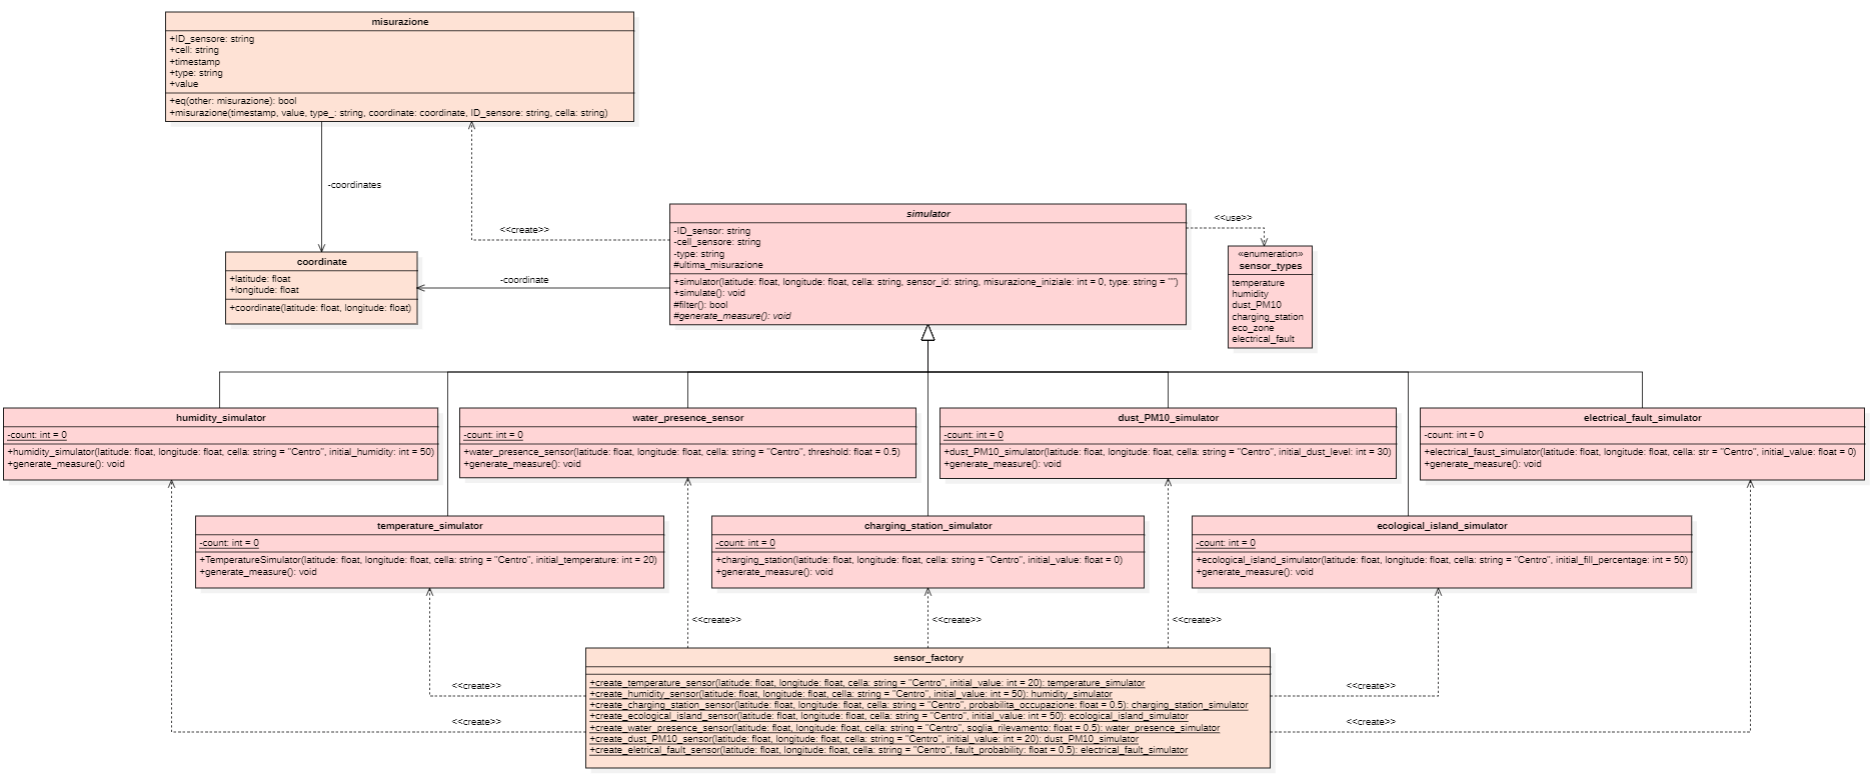
\includegraphics[width=1\textwidth]{../Images/SpecificaTecnica/simulatoriSensori.PNG}
    \caption{Modulo writers - innovacity}
    \label{fig: fdsd}
\end{figure}

Questo modulo si occupa della scrittura e/o invio di informazioni a diverse tipologie di servizi e vuole essere completamentemente indipendendente e non influenzato dal modulo della simulazione dei sensori cosi da poter consentire un suo riutilizzo.

\paragraph{Design pattern Strategy + Composite:}
Il modulo presenta un interfaccia \textit{Writer} che offre il metodo di scrittura \textit{write()} di oggetti di tipo \textit{Writable}.
Questo metodo è implementato da diverse classi concrete che rappresentano i vari servizi a cui è possibile inviare le informazioni.
Questo approccio implementa il design pattern \textit{Strategy} per la scrittura dei dati su diverse piattaforme/servizi e il design pattern \textit{Composite} per la gestione di più servizi a cui scrivere contemporaneamente in modo completamentemente indifferenziato dalla scrittura ad un singolo servizio.
Nello specifico sono state implentate tre strategie di scrittura:la prima, (\textit{KafkaWriter}), atta a permettere al simulatore di inviare messaggi a Kafka,  la seconda (\textit{StdOutWriter}) atta a permettere di stampare i \textit{Writable}su terminale e la terza (\textit{ListWriter}) per il salvataggio su una lista degli oggetti \textit{Writable}.
L'utilizzo del design pattern Composite e Strategy in questo caso ha diverse motivazioni:
\begin{itemize}
    \item \textbf{Gestione uniforme dei servizi}: Il pattern Strategy consente di definire una famiglia di algoritmi, incapsularli e renderli intercambiabili. In questo caso, i servizi di scrittura sono trattati come algoritmi intercambiabili, consentendo di scrivere informazioni su diversi servizi senza dover conoscere i dettagli di implementazione di ciascuno.
    \item \textbf{Gestione gerarchica dei servizi}: Il pattern Composite consente di trattare gli oggetti singoli e le loro composizioni (gruppi di oggetti) allo stesso modo. Nel contesto del modulo, potrebbe esserci la necessità di gestire non solo singoli servizi, ma anche gruppi di servizi. Ad esempio, potrebbe essere utile inviare informazioni contemporaneamente a diversi servizi, come un database, un file di log e un servizio di notifica. Il Composite consente di comporre questi servizi in modo gerarchico e trattarli uniformemente.
\end{itemize}

\paragraph{Design pattern Object Adapter:}
Nello specifico, la classe \textit{KafkaWriter} realizza la sua funzionalità attraverso l'utilizzo del design pattern \textit{Adapter}, nella sua variante \textit{Object Adapter}. Tale scelta è stata motivata dall'impiego della classe \textit{Producer} della libreria \textit{confluent\_kafka}, la quale potrebbe subire variazioni non controllabili da noi. Per garantire la capacità di rispondere prontamente a tali cambiamenti senza dover modificare la classe \textit{KafkaWriter} o altri parti di sistema, si è optato per l'utilizzo di questo pattern, trasferendo così la complessità derivante da tali modifiche proprio nell'adapter.
Inoltre grazie all'interfaccia \textit{KafkaTarget}, si è garantita la possibilità di estendere il sistema con nuovi metodi di scrittura su Kafka o l'utilizzo di nuove librerie senza dover modificare la classe \textit{KafkaWriter} ma solamente aggiungendo una nuova classe adapter che implementi \textit{KafkaTarget}.



\paragraph{Classi: metodi e attributi}

\begin{itemize}
    \item{\textbf{Interfaccia: \textit{Writable}}}
    \begin{itemize}
        \item\textbf{Metodi}: 
        \begin{itemize}
            \item \textbf{to\_json(): [public, abstract]} - Metodo astratto che deve essere implementato nelle sottoclassi per convertire l'oggetto in una stringa JSON.
        \end{itemize}
        \item\textbf{Note}:
        \begin{itemize}
            \item L'interfaccia \textit{Writable} definisce un insieme di metodi che una classe deve implementare perchè possa essere utilizzata dalle strategie di scrittura.
        \end{itemize}
    \end{itemize}
    \item{\textbf{Interfaccia: \textit{Writer}}}
     \begin{itemize}
        \item \textbf{Metodi:}
         \begin{itemize}
            \item \textbf{write(to\_write: Writable): None [public, abstract]} - Metodo astratto che deve essere implementato nelle sottoclassi per scrivere un oggetto Writable.
        \end{itemize}
        \item\textbf{Note}:
        \begin{itemize}
            \item L'interfaccia \textit{Writer} definisce un insieme di metodi che una classe deve implementare perchè possa essere utilizzata come strategia di scrittura;
            \item Rappresenta l'interfaccia "Component" del pattern \textit{Composite} che descrive le operazioni comuni sia agli elementi semplici che a quelli complessi dell'albero.
        \end{itemize}
    \end{itemize}
    \item{\textbf{Classe: \textit{StdoutWriter}}}
    \begin{itemize}
    \item\textbf{Attributi}:
        \begin{itemize}
        \item \textbf{lock:threading.Lock [private]} - Lock per garantire l'accesso esclusivo alla stampa ed un esecuzione Thread safe.
    \end{itemize}
    \item \textbf{Metodi: }
    \begin{itemize}
        \item \textbf{write(to\_write: Writable): None [public]} - Stampa l'oggetto Writable come stringa JSON nella console;
    \end{itemize}
    \item\textbf{Note}:
        \begin{itemize}
            \item La classe è una strategia di scrittura del pattern \textit{Strategy} ma anche la componente "Leaf" del pattern \textit{Composite}, ovvero l'elemento base che non ha sottoelementi.
        \end{itemize}
    \end{itemize}
    \item{\textbf{Classe: \textit{ListWriter}}}
    \begin{itemize}
    \item\textbf{Attributi}:
        \begin{itemize}
        \item \textbf{data\_list:list [private]} - Lista per memorizzare gli oggetti Writable.
        \item \textbf{lock:threading.Lock [private]} - Lock per garantire l'accesso esclusivo alla lista ed un esecuzione Thread safe.
    \end{itemize}
    \item \textbf{Metodi: }
    \begin{itemize}
        \item \textbf{write(to\_write: Writable): None [public]} - Aggiunge l'oggetto Writable alla lista.
        \item \textbf{get\_data\_list(): list [public]} - Restituisce la lista di oggetti Writable.
    \end{itemize}
    \item\textbf{Note}:
        \begin{itemize}
            \item La classe è una strategia di scrittura del pattern \textit{Strategy} ma anche la componente "Leaf" del pattern \textit{Composite}, ovvero l'elemento base che non ha sottoelementi.
        \end{itemize}
    \end{itemize}
    \item{\textbf{Classe: \textit{KafkaWriter}}}
    \begin{itemize}
    \item\textbf{Attributi}:
        \begin{itemize}
        \item \textbf{lock:threading.Lock [private]} - Lock per garantire l'accesso esclusivo alla scrittura su Kafka ed un esecuzione Thread safe.
        \item \textbf{kafka\_target:KafkaTarget [private]} - Riferimento ad un implementazione di KafkaTarget per effettuare l'effettiva scrittura in Kafka tramite librerie.
    \end{itemize}
    \item \textbf{Metodi: }
    \begin{itemize}
        \item \textbf{write(to\_write: Writable): None [public]} - Scrive l'oggetto Writable come stringa JSON su Kafka.
    \end{itemize}
    \item\textbf{Note}:
        \begin{itemize}
            \item La classe è una strategia di scrittura del pattern \textit{Strategy} ma anche la componente "Leaf" del pattern \textit{Composite}, ovvero l'elemento base che non ha sottoelementi.
            \item La costruzione dell'oggetto KafkaWriter richiede un riferimento ad un oggetto che implementi l'interfaccia KafkaTarget.
        \end{itemize}
    \end{itemize}
    \item{\textbf{Classe: \textit{CompositeWriter}}}
    \begin{itemize}
    \item\textbf{Attributi}:
        \begin{itemize}
        \item \textbf{writers:Writer* [protected]} - Lista di oggetti Writer.
    \end{itemize}
    \item \textbf{Metodi: }
    \begin{itemize}
        \item \textbf{add\_writer(writer: Writer): CompositeWriter [public]} - Aggiunge un oggetto Writer alla lista di writers.
        \item \textbf{add\_kafkaConfluent\_writer(topic: str, host: str, port: int): CompositeWriter [public]} - Crea un KafkaWriter con un KafkaConfluentAdapter e lo aggiunge alla lista di writers.
        \item \textbf{add\_stdOut\_writer(): CompositeWriter [public]} - Crea un StdoutWriter e lo aggiunge alla lista di writers.
        \item \textbf{add\_list\_writer(writer\_list: ListWriter): CompositeWriter [public]} - Aggiunge un ListWriter alla lista di writers.
        \item \textbf{remove\_writer(writer: Writer): None [public]} - Rimuove un Writer dalla lista di writers.
        \item \textbf{write(to\_write: Writable): None [public]} - Chiama il metodo write su ogni Writer nella lista di writers passando come attributo il \textit{Writable} ricevuto.
    \end{itemize}
    \item\textbf{Note}:
        \begin{itemize}
            \item La classe è la componente "Composite" del pattern \textit{Composite}, ovvero l'elemento che può avere sottoelementi;
            \item Dopo aver ricevuto una richiesta, il contenitore (detto compisite) delega il lavoro ai suoi sottoelementi:foglie o altri contenitori.
        \end{itemize}
    \end{itemize}
    \item{\textbf{Interfaccia: \textit{KafkaTarget}}}
    \begin{itemize}
    \item \textbf{Metodi: }
    \begin{itemize}
        \item \textbf{write\_to\_kafka(data: str): None [public, abstract]} - Metodo astratto che deve essere implementato nelle sottoclassi per scrivere dati su Kafka.
    \end{itemize}
    \item\textbf{Note}:
        \begin{itemize}
            \item La classe è una interfaccia che fornisce un contratto per le operazioni di scrittura e invio a Kafka.
            \item Rappresenta il componente Target del pattern \textit{Object Adapter}.
        \end{itemize}
    \end{itemize}
    \item{\textbf{Classe: \textit{KafkaConfluentAdapter}}}
    \begin{itemize}
    \item\textbf{Attributi}:
        \begin{itemize}
        \item \textbf{topic:str [private]} - Il topic su cui scrivere in Kafka.
        \item \textbf{producer:Producer [private]} - Il producer Kafka per inviare messaggi.
    \end{itemize}
    \item \textbf{Metodi: }
    \begin{itemize}
        \item \textbf{write\_to\_kafka(data: str): None [public]} - Scrive i dati su Kafka.
    \item\textbf{Note}:
        \begin{itemize}
            \item La classe è un'implementazione concreta dell'interfaccia KafkaTarget, utilizzando la libreria confluent-kafka per interagire con Kafka;
            \item Rappresenta il componente "Adapter" del pattern \textit{Object Adapter}.
            \item Il Producer kafka rappresenta la componente "service" del pattern \textit{Object Adapter}.
        \end{itemize}
    \end{itemize}
\end{itemize}

\subsubsection{Modulo Threading/Scheduling}
Questo modulo si propone di gestire la logica di pianificazione per il recupero dei dati dai simulatori dei sensori e di inviare/scrivere tali dati utilizzando gli "Writers". Funge da orchestratore per i due moduli appena descritti, offrendo la possibilità di configurare la frequenza di campionamento o il numero di misurazioni da eseguire. Inoltre, incorpora una logica di ottimizzazione, simile a quella impiegata dai microcontrollori dei sensori nella realtà, al fine di evitare la trasmissione di dati ridondanti, inviando solo i cambiamenti di stato dei sensori.

\paragraph*{Dependecy Inversion principle}
Il modulo è stato progettato per rispettare il principio di inversione delle dipendenze. Infatti, la classe \textit{SimulatorThreadPool} è stata progettata per essere indipendente dalla libreria di gestione dei thread utilizzata, consentendo di sostituire la libreria di gestione dei thread senza dover modificare il codice di \textit{SimulatorThreadPool}.
Inoltre, i componenti del modulo sono progettati per essere indipendenti dai dettagli di implementazione dei simulatori e dei writers, consentendo di sostituire i simulatori e i writers senza dover modificare il codice.

\paragraph{Design pattern Composite:}
Come per il modulo di scrittura anche questo è sviluppato secondo il pattern Composite che permette di gestire un singolo Thread di esecuzione o un gruppo di Thread in modo uniforme.
\paragraph{Design pattern Object Adapter:}
Inoltre, considerando l'impiego di più thread per un esecuzione parallela, per delegare l'orchestrazione delle operazioni, si è fatto ricorso alle ThreadPool. Al fine di evitare modifiche dirette al codice di \textit{SimulatorThreadPool}, è stato adottato il pattern \textit{Object Adapter} per adattare la ThreadPool di Python a un'interfaccia comune con cui \textit{SimulatorThreadPool} possa interagire. Questo approccio consente di modificare la logica o la libreria utilizzata per la gestione dei thread senza richiedere modifiche al codice di \textit{SimulatorThreadPool}, ma semplicemente aggiungendo una nuova classe adapter che implementi \textit{ThreadPoolTarget}.


Un'altra implementazione del pattern \textit{Object Adapter} viene impiegata per adattare gli oggetti \textit{Misurazione} del modulo \textit{Simulatori} agli oggetti \textit{Writable} del modulo \textit{Writers}. La classe \textit{AdapterMisurazione}, implementando l'interfaccia \textit{Writable}, fornisce un'implementazione del metodo \textit{to\_json()} che consente di convertire un oggetto \textit{Misurazione} nel formato JSON, compatibile e riconosciuto da Kafka.
\ref*{sec:formatoMessaggi}


\paragraph{Classi: metodi e attributi}

\begin{itemize}
 \item{\textbf{Interfaccia: \textit{ComponentSimulatorThread}}}
    \begin{itemize}
        \item \textbf{Metodi: }
        \begin{itemize}
            \item \textbf{run(): None [public, abstract]} - Metodo astratto che deve essere implementato nelle sottoclassi per definire il comportamento del thread quando viene avviato.
            \item \textbf{task(): None [public, abstract]} - Metodo astratto che deve essere implementato nelle sottoclassi per definire il compito specifico che il thread deve eseguire.
            \item \textbf{stop(): None [public, abstract]} - Metodo astratto che deve essere implementato nelle sottoclassi per definire come fermare il thread.
        \end{itemize}
        \item\textbf{Note}:
            \begin{itemize}
                \item Eredita le proprietà e i metodi della classe Thread della \textit{Standard Library};
                \item \textit{ComponentSimulatorThread} è un interfaccia di threading per la simulazione sensori, fornendo un contratto per le operazioni di avvio, esecuzione del compito e arresto;
                \item Rappresenta il componente "Component" del pattern \textit{Composite},descrive le operazioni comuni sia ai singoli Thread sia alle composizioni;
                \item L'utilizzatore dei simulatori può lavorare allo stesso modo con elementi semplici (Singoli Thread) o complessi dell'albero (Insiemi di Thread in forma di albero).
            \end{itemize}
    \end{itemize}
    \item{\textbf{Classe: \textit{SimulatorThread}}}
    \begin{itemize}
    \item\textbf{Attributi}:
        \begin{itemize}
        \item \textbf{simulator:Simulator [private]} - Il simulatore da utilizzare per generare i dati.
        \item \textbf{frequency:float [private]} - La frequenza con cui generare i dati.
        \item \textbf{is\_running:bool [private]} - Flag per controllare se il thread è in esecuzione.
        \item \textbf{data\_to\_generate:int [private]} - Il numero di dati da generare.
        \item \textbf{writers:Writer [private]} - L'oggetto Writer per scrivere i dati generati. (Singolo o albero)
        \end{itemize}
    \item \textbf{Metodi: }
        \begin{itemize}
        \item \textbf{run(): None [public]} - Avvia il thread del simulatore.
        \item \textbf{task(): None [public]} - Definisce il compito specifico che il thread deve eseguire, contiene la logica per generare il numero di misurazioni richieste con l'intervallo specificato alla costruzione.
        Inoltre evita l'invio di misurazioni consecutive uguali cosi da evitare ulteriore sovraccarico di dati ridondanti e deducibili inviando agli Writers solo i cambi di stato del sensore da cui acquisisce la misurazione.
        All'interno del metodo la misurazione restituita dal simulatore viene adattata ad un oggetto \textit{Writable} tramite \textit{AdapterMisurazione} ed inviata agli \textit{Writers}.
        \item \textbf{stop(): None [public]} - Ferma il thread del simulatore.
        \end{itemize}
    \item\textbf{Note}:
        \begin{itemize}
            \item La classe è un'implementazione concreta dell'interfaccia ComponentSimulatorThread, utilizzando un oggetto Simulator per generare dati a una certa frequenza e un oggetto Writer per scrivere i dati generati.
            \item Rappresenta il componente Leaf del pattern \textit{Composite}.
            \item Se data\_to\_generate < 0 => Genera misurazioni finchè il thread non viene interroto dall'esterno.
            \item Sebbene i simulatori non siano considerati dalla proponente parte del prodotto, la logica di ottimizzazione per inviare solo i cambi di stato dei sensori viene implementata nella realtà IoT, quindi si è deciso di replicarla. Di conseguenza, è stata presa la decisione di replicarla. È importante notare che questa logica non è incorporata nel Simulatore del sensore, il quale ha unicamente il compito semantico di generare dati come un vero sensore. Invece, essa è implementata nel SimulatorThread, il quale agisce in modo simile a un microcontrollore, responsabile sia della gestione dell'intervallo di campionamento che della logica per l'invio delle misurazioni.
            \item Nel corso dello sviluppo futuro, potrebbe risultare vantaggioso considerare l'implementazione di un pattern \textit{Strategy} per gestire la strategia/criterio di invio dei dati, che possa distinguere tra un invio continuo e la trasmissione solo in caso di cambiamenti di stato. Tuttavia, al momento della decisione, si è optato per non includerlo al fine di evitare un'eccessiva complessità nell'architettura, nota come sovraingegnerizzazione. Tale scelta è stata dettata dalla volontà di mantenere un equilibrio tra la completezza del sistema e la sua semplicità, favorendo un'implementazione più diretta e immediata delle funzionalità richieste.
        \end{itemize}
    \end{itemize}
    \item{\textbf{Classe: \textit{AdapterMisurazione}}}
    \begin{itemize}
    \item\textbf{Attributi}:
        \begin{itemize}
        \item \textbf{misurazione:Misurazione [private]} - L'oggetto Misurazione da adattare.
    \end{itemize}
    \item \textbf{Metodi: }
    \begin{itemize}
        \item \textbf{to\_json(): dict [public]} - Converte l'oggetto Misurazione in un dizionario JSON conforme a quanto definito in \ref{sec:formatoMessaggi}.
        \item \textbf{from\_json(json\_data: dict): Misurazione [staticmethod, public]} - Crea un oggetto Misurazione da un dizionario JSON.
    \end{itemize}
    \item\textbf{Note}:
        \begin{itemize}
            \item La classe è un'implementazione concreta dell'interfaccia Writable. Fornisce metodi per convertire un oggetto Misurazione in un formato JSON e viceversa.
            \item Rappresenta la come componente "Adapter" del pattern \textit{Object Adapter}.
        \end{itemize}
    \end{itemize}
    \item{\textbf{Classe: \textit{SimulatorExecutorFactory}}}
    \begin{itemize}
    \item\textbf{Attributi}:
        \begin{itemize}
        \item \textbf{simulator\_executor:SimulatorThreadPool [private]} - L'executor del simulatore per gestire l'esecuzione dei Thread dei simulatori.
    \end{itemize}
    \item \textbf{Metodi: }
    \begin{itemize}
        \item \textbf{add\_simulator(simulator: Simulator, writers: Writer, frequency: float, data\_to\_generate: int): SimulatorExecutorFactory [public]} - Aggiunge un simulatore all'executor.
        \item \textbf{add\_simulator\_thread(thread\_simulator: ComponentSimulatorThread): SimulatorExecutorFactory [public]} - Aggiunge un thread di simulatore all'executor.
        \item \textbf{run(): None [public]} - Avvia tutti i simulatori nell'executor.
        \item \textbf{stop(): None [public]} - Ferma tutti i simulatori nell'executor.
        \item \textbf{task(): None [public]} - Avvia tutti i simulatori nell'executor.
    \end{itemize}
    \item\textbf{Note}:
        \begin{itemize}
            \item La classe è un'implementazione concreta dell'interfaccia ComponentSimulatorThread, utilizzando un oggetto SimulatorThreadPool per gestire l'esecuzione di vari simulatori.
            \item 
        \end{itemize}
    \end{itemize}
    \item{\textbf{Classe: \textit{SimulatorThreadPool}}}
    \begin{itemize}
    \item\textbf{Attributi}:
        \begin{itemize}
        \item \textbf{simulators:List[ComponentSimulatorThread] [private]} - La lista dei \textit{ComponentSimulatorThread} da eseguire. (Singoli Thread o alberi di Thread)
        \item \textbf{thread\_pool:ThreadPoolTarget [private]} - Thread pool per gestire l'esecuzione parallela dei simulatori.
    \end{itemize}
    \item \textbf{Metodi: }
    \begin{itemize}
        \item \textbf{run\_all(): None [public]} - Avvia tutti i simulatori nel thread pool, utilizzando l'interfaccia fornita da \textit{ThreadPoolTarget} per l'esecuzione controllata di attività in parallelo.
        \item \textbf{stop\_all(): None [public]} - Ferma tutti i simulatori nel thread pool, utilizzando l'interfaccia fornita da \textit{ThreadPoolTarget} per l'esecuzione controllata di attività in parallelo..
        \item \textbf{append\_simulator(simulator: ComponentSimulatorThread): None [public]} - Aggiunge un \textit{ComponentSimulatorThread} al thread pool.
        \item \textbf{start\_simulator(simulator: ComponentSimulatorThread): None [private,static]} - Avvia un \textit{ComponentSimulatorThread}.
        \item \textbf{stop\_simulator(simulator: ComponentSimulatorThread): None [private,static]} - Ferma un \textit{ComponentSimulatorThread}.
    \end{itemize}
    \item\textbf{Note}:
        \begin{itemize}
            \item La classe gestisce un pool di thread per l'esecuzione di vari simulatori, utilizzando un oggetto \textit{ThreadPoolTarget} per gestire l'esecuzione dei simulatori;
            \item I metodi \textit{run\_all()} e \textit{stop\_all()} utilizzano l'interfaccia fornita da \textit{ThreadPoolTarget} per mappare rispettivamente la funzione statica \textit{start\_simulator()} e \textit{stop\_simulator()} per ogni \textit{ComponentSimulatorThread} in \textit{simulators}.
            \item Grazie all'utilizzo di \textit{ThreadPoolTarget} è possibile estendere il sistema con nuovi metodi di esecuzione controllata di attività in parallelo o l'utilizzo di nuove librerie senza dover modificare la classe \textit{SimulatorThreadPool} ma solamente aggiungendo una nuova classe adapter che implementi \textit{ThreadPoolTarget}.
        \end{itemize}
    \end{itemize}
    \item{\textbf{Classe: \textit{ThreadPoolTarget}}}
    \begin{itemize}
    \item\textbf{Metodi: }
    \begin{itemize}
        \item \textbf{map(func, iterable): [abstractmethod]} - Un metodo astratto che deve essere implementato nelle sottoclassi. Questo metodo applica la funzione `func` a ogni elemento nell'`iterable`.
    \end{itemize}
    \item\textbf{Note}:
        \begin{itemize}
            \item L'interfaccia rappresenta la componente "Target" del pattern \textit{Object Adapter} fornendo un contratto per le operazioni di esecuzione controllata di attività in parallelo.
         \end{itemize}
    \end{itemize}
    \end{itemize}
    \item{\textbf{Classe: \textit{ThreadPoolExecutorAdapter}}}
    \begin{itemize}
    \item\textbf{Attributi}:
        \begin{itemize}
        \item \textbf{executor:concurrent.futures.ThreadPoolExecutor [private]} - L'executor della thread pool per gestire l'esecuzione dei thread.
    \end{itemize}
    \item \textbf{Metodi: }
    \begin{itemize}
        \item \textbf{map(func, iterable): [public]} - Applica la funzione `func` a ogni elemento nell' `iterable` utilizzando l'executor del thread pool.
    \end{itemize}
    \item\textbf{Note}:
        \begin{itemize}
            \item La classe è un'implementazione concreta dell'interfaccia ThreadPoolTarget, utilizzando un oggetto concurrent.futures.ThreadPoolExecutor per gestire l'esecuzione dei thread.
            \item Rappresenta il componente "Adapter" del pattern \textit{Object Adapter}.
            \item Adatta l'oggetto ThreadPoolExecutor dalla libreria \textit{concurrent.futures}
            \item Al momento della costruzione deve essere fornito il parametro intero "workers" ovvero
            Il numero massimo di thread che è possibile utilizzare per eseguire le task indicate.
        \end{itemize}
    \end{itemize}




\end{itemize}


